\documentclass[12pt]{iopart}
\pdfminorversion=4
\usepackage{graphicx}
%Uncomment next line if AMS fonts required
%\usepackage{iopams}  
\usepackage{myphysics} %units, particles and misc definitions from ATLAS 
\usepackage{graphicx}  %\includegraphics...

\begin{document}

\title[Electroweak phyiscs at the LHC]{Electroweak physics at the LHC}
\author{J Berryhill$^1$ and A Oh$^2$}

\address{$^1$ Fermi National Accelerator Laboratory, Batavia, IL, USA}
\address{$^2$ School of Physics and Astronomy, University of Manchester, Manchester, UK}

%\ead{submissions@iop.org}
%\vspace{10pt}
%\begin{indented}
%\item[]February 2014
%\end{indented}

\begin{abstract}
The Large Hadron Collider (LHC) has completed in 2012 its first
running phase and the experiments have collected data sets of pp
collisions at center-of-mass energies of 7 and 8 TeV with an
integrated luminosity of about 5ifb and 20ifb, respectively.  Analyses
of these data sets have produced a rich set of results in the
electroweak sector of the standard model. This article reviews the
status of electroweak measurements of the ATLAS and CMS experiments at
the LHC and discusses phenomenological developments in the electroweak
sector.
\end{abstract}

% Uncomment for PACS numbers
\pacs{00.00, 20.00, 42.10}
%
% Uncomment for keywords
\vspace{2pc}
\noindent{\it Keywords}: XXX, YYY, ZZZ
%
% Uncomment for Submitted to journal title message
\submitto{\jpg}
%
% Uncomment if a separate title page is required
\maketitle
% 
% For two-column output uncomment the next line and choose [10pt] rather than [12pt] in the \documentclass declaration
%\ioptwocol
%


\section{Introduction}
\subsection{Motivation to study the electroweak sector}
\subsection{Electroweak physics at hadron colliders}
\subsection{LHC physics program}
\subsection{Electroweak challenges for Run 2 and beyond}

\section{Theory overview and recent developments}
\subsection{PDF and electroweak observables (V+jets, phi*)}
\subsection{Electroweak NLO corrections}
\subsection{Anomalous gauge couplings and effective field theory}
\subsection{Oblique corrections, constructed observables}


\section{Inclusive boson production}
\subsection{Drell-Yan production}
ATLAS high-mass Drell--Yan 7 TeV~\cite{Aad:2013iua} 

ATLAS low-mass Drell-Yan 7 TeV~\cite{Aad:2014qja}

ATLAS Z PT 7 TeV~\cite{Aad:2014xaa}

ATLAS Z phistar 7 TeV~\cite{Aad:2012wfa}

CMS Drell--Yan 7 TeV~\cite{Chatrchyan:2013tia}

CMS Drell--Yan 8 TeV~\cite{CMS:2014jea}

CMS angular coefficients 8 TeV~\cite{Khachatryan:2015paa}

CMS Z PT and rapidity 8 TeV~\cite{Khachatryan:2015oaa}

\begin{figure}[p]
    \centering
    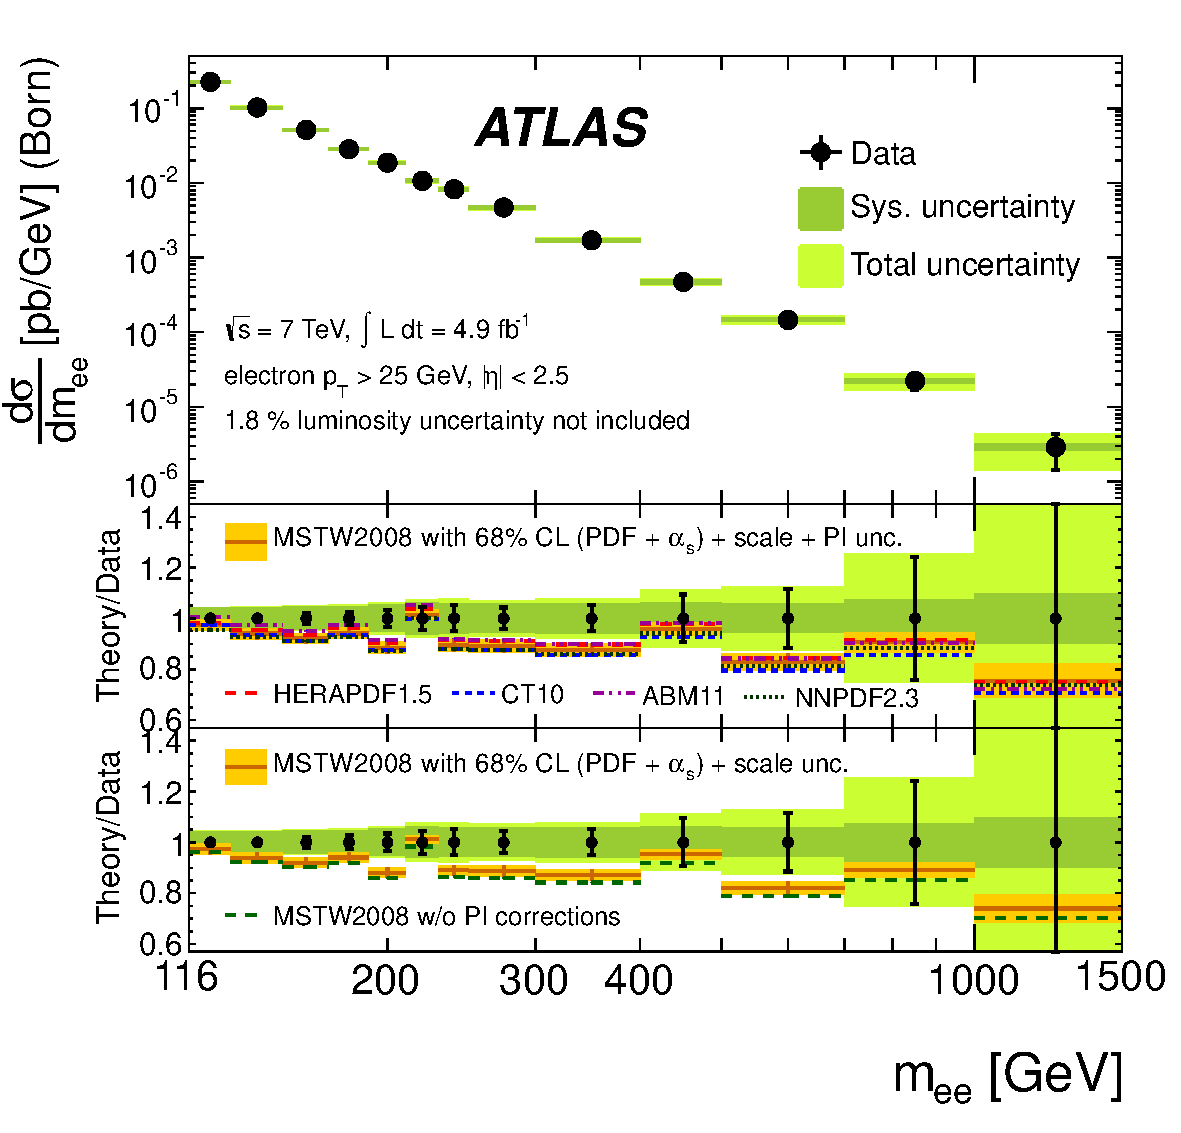
\includegraphics[height=0.3\textheight]{atlas_drellyan7tev}
    \caption{Measured differential cross-section at the Born level within the fiducial region (electron $p_T > 25$ GeV and $|\eta| < 2.5$) with statistical, systematic, and combined statistical and systematic (total) uncertainties, excluding the 1.8\% uncertainty on the luminosity. The measurement is compared to FEWZ 3.1 calculations at NNLO QCD with NLO electroweak corrections using the $G_{\mu}$ electroweak parameter scheme. The predictions include an additional small correction from single-boson production in which the final-state charged lepton radiates a real W or Z boson. On the left, in the upper ratio plot, the photon-induced (PI) corrections have been added to the predictions obtained from the MSTW2008, HERAPDF1.5, CT10, ABM11 and NNPDF2.3 NNLO PDFs, and for the MSTW2008 prediction the total uncertainty band arising from the PDF, $\alpha_s$, renormalisation and factorisation scale, and photon-induced uncertainties is drawn. The lower ratio plot shows the influence of the photon-induced corrections on the MSTW2008 prediction, the uncertainty band including only the PDF, $\alpha_s$ and scale uncertainties. On the right, the results are shown for a restricted range of $m_{ee}$.}
    \label{fig:atlas_drellyan7tev}
\end{figure}

\begin{figure}[p]
    \centering
    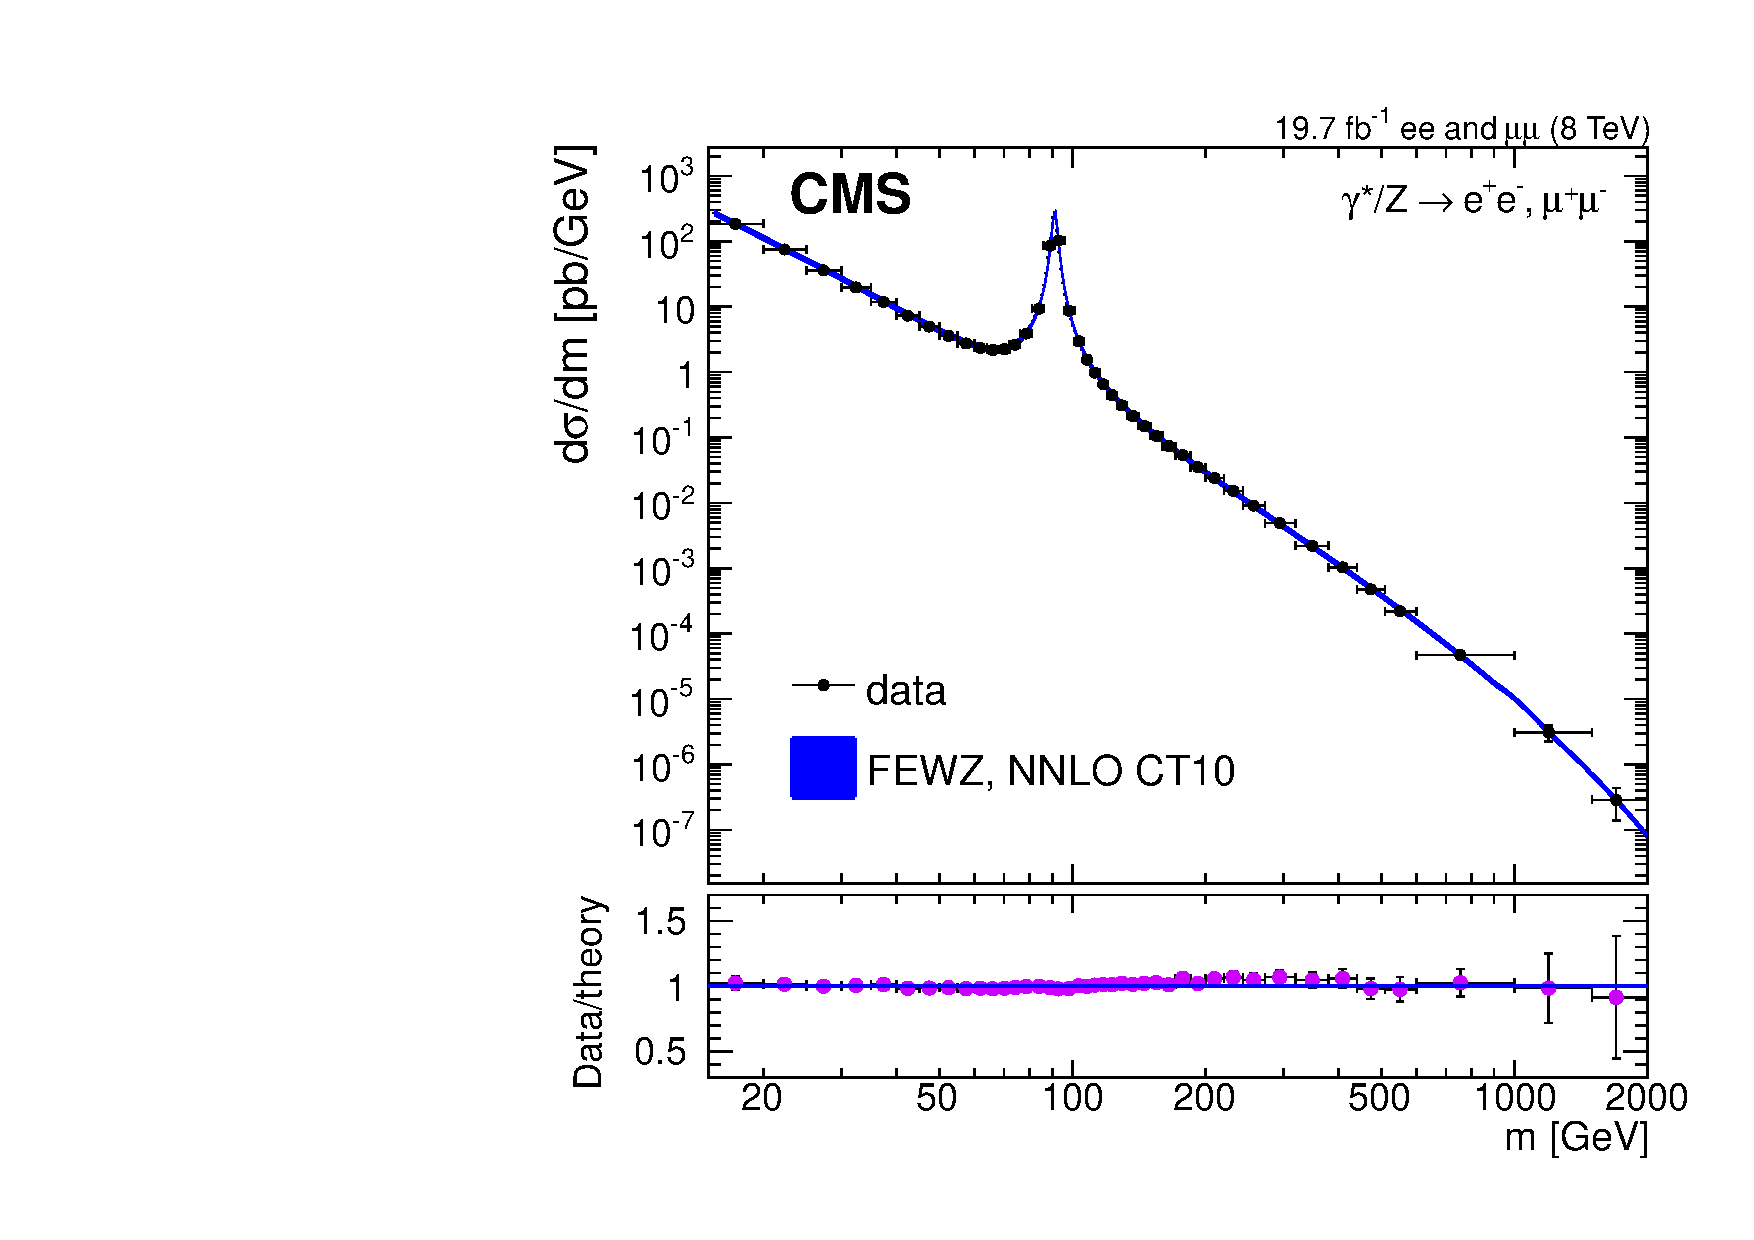
\includegraphics[height=0.3\textheight]{cms_drellyan8tev}
    \caption{}
    \label{fig:cms_drellyan8tev}
\end{figure}


\subsection{Inclusive di-boson production}

ATLAS Wgamma Zgamma 7 TeV~\cite{Aad:2013izg}

CMS Wgamma/Zgamma 7 TeV~\cite{Chatrchyan:2013fya}

CMS Znngamma 7 TeV~\cite{Chatrchyan:2013nda}

CMS Zgamma 8 TeV~\cite{Khachatryan:2015kea}


ATLAS simultaneous tt/WW/Z cross section 7 TeV~\cite{Aad:2014jra}

ATLAS WW 7 TeV~\cite{ATLAS:2012mec}

ATLAS $WW+WZ$ cross section 7 TeV~\cite{Aad:2014mda}

ATLAS WW 8 TeV~\cite{ATLAS-CONF-2014-033}

CMS WW2l2n 7 TeV~\cite{Chatrchyan:2013yaa}

CMS WWlnjj 7 TeV~\cite{Chatrchyan:2012bd}

CMS WW/ZZ 8 TeV~\cite{Chatrchyan:2013oev}

CMS WW2l2n 8 TeV (CMS-PAS-SMP-14-016, to be published)


ATLAS WZ 7 TeV~\cite{Aad:2012twa}

CMS VZ 8 TeV~\cite{Chatrchyan:2014aqa}

CMS WZ at 7+8 TeV (CMS-PAS-SMP-12-006, to be published)

\subsubsection{ZZ production}
\label{sss-ZZprod}

lala

\subsubsection{ZZ production}
\label{sss-ZZprod}

%short intro
The production of \ZZ in proton-proton collisions has been one of the first di-boson 
processes measured at the LHC. The SM process is and an important and irreducible
background to resonance searches and Higgs production. The production at leading
order is dominated by quark anti-quark annihilation in the $t$ and $u$-channel,
whereas the $s$-channel process is forbidden in the SM 
(see also Figure~\ref{fig:sss-ZZprod-LOdiagrams}). The gluon fusion process 
contributes about 6\% to the total production cross section. 

%FIGURE LO ZZ DIAGRAM
\begin{figure}[htbp]
  \begin{center}
  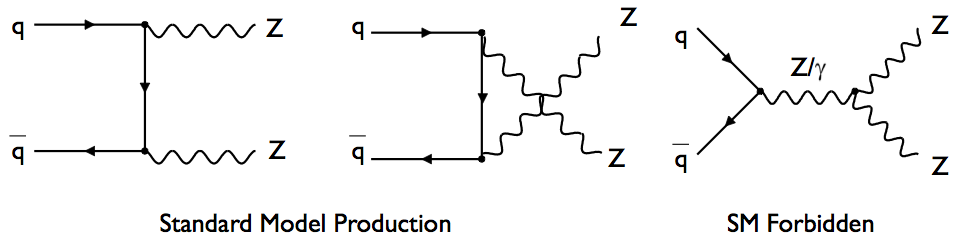
\includegraphics[width=0.9\textwidth]{figures/sss-inclboson-diboson-zzprod-zzdiagram.png}
  \caption{Leading order Feynman diagrams of \ZZ production in the dominant 
  \qqbar\ channel. The \ZZ\ production via the $s$-channel is not allowed in the SM.}
\label{fig:sss-ZZprod-LOdiagrams}
\end{center}
\end{figure}

%decay channels
Precision measurements use the leptonic decay modes of the $Z$ to reduce the impact of
QCD backgrounds. 
The four lepton final state provides an almost background free signature, at the
expense of a relatively small branching ratio 
$BR(ZZ) \to \ll\ll = 0.101^2 \cdot {4 \over 9} = 0.0045$~\cite{PDG}.  
The di-lepton and missing energy channel can exploit the one order of magnitude
higher branching ratio of 
$BR(\ZZ \to \ll\vv) = 0.101 \cdot 0.20 \cdot 2 \cdot {2 \over 3} = 0.0269$, 
at the expense of high background levels.

%analysis CMS and ATLAS.
%ATLAS ZZ 7 TeV~\cite{Aad:2012awa}
%CMS ZZ4l 8 TeV~\cite{Khachatryan:2014dia}
%CMS ZZ4l 7 TeV~\cite{Chatrchyan:2012sga}
%CMS ZZ2l2nu 7+8 TeV~\cite{Khachatryan:2015pba}
The ATLAS collaboration has published results on the $7\TeV$ data-set 
in the $\ll\ll$ and $\ll\vv$ final state~\cite{Aad:2012awa}, and at
$13\TeV$ in the $\ll\ll$ final state~\cite{Aad:2015zqe}. The CMS collaboration
has analysed the full 7 and $8\TeV$ data sets in both 
the $\ll\ll$~\cite{Chatrchyan:2012sga,Khachatryan:2014dia} and 
$\ll\vv$ final state~\cite{Khachatryan:2015pba}.

%Theoretical calculations
% NLO alpha_s arXiv:1105.0020
% NLO alpha_EKW arXiv:1305.5402,arXiv:1307.4331
Theoretical predictions for $\ZZ$ production are available 
at NLO in $\alpha_s$~\cite{arXiv:1105.0020}. In addition, electroweak 
corrections at NLO have been calculated~\cite{arXiv:1305.5402,arXiv:1307.4331}. 

% Z->llll
%Selections
The event selection for the $\ll\ll$ final state requires exactly four leptons 
fulfilling a set of cuts on kinematic quantities. ATLAS and CMS use similar criteria 
as listed in detail in Table~\ref{tab:sss-ZZprod-cuts}. While ATLAS uses $l=e,\mu$,
CMS includes also $\Z\to\tautau$ with subsequent hadronic and leptonic $\tau$
decays. ATLAS uses in addition forward leptons outside the ID tracker
to increase the acceptance by 6\% for electrons and 10\% for muons.
%Backgrounds
The $\ll\ll$ channels offers the cleanest event sample with a background level
of only $2-3\%$ from $\Z+jets$, $\tt$, and di-boson events. 
The background is estimated from data by control regions with looser selection
criteria. 

% Z->llvv
%Selections
Events in the $\ll\vv$ final state are characterized by exactly two leptons 
and missing energy. The event selection requires a leptonic $\Z$ candidate and
missing energy in the event. Both experiments used refined observables of
missing energy with additional information to improve the rejection 
against instrumental background. 
%Backgrounds 
The background level is in the same order
as the signal and substantially higher then for $\ll\ll$ .
Main background sources are $\V+jets$, $\tt$ and di-boson production. 
ATLAS and CMS use data driven techniques to constrain the 
dominant background sources.

% Results at the end?
% xsec
Besides the total cross section for the $pp \to \ZZ$ production process, both
experiments measure also fiducial and differential cross sections. The results are 
summarized in Tabel~\ref{tab:sss-ZZprod-cross-sections}. ATLAS and CMS
use different definitions of the fiducial phase space which needs to be taken into
account to make a direct comparison is possible.
For the total cross section a slightly different mass range for the $\Z$ mass range is
used, where CMS uses a wider range of $60\GeV < \mZ < 120\GeV$ then ATLAS with 
$66\GeV < \mZ < 116\GeV$, which contributes to the difference in the quoted predicted
cross section. Good agreement of experimental and theoretical cross section 
values is observed. 


\begin{table}[htp]
\begin{center}
\resizebox{\textwidth}{!}{
\begin{tabular}{|c|c|c|c|c|c|}
 \hline
 Experiment & decay channel     & \rts & measured $\sigma_{total}$ $[\pb]$                                  & predicted $\sigma_{total}$ $[\pb]$& reference                    \\
 \hline
 ATLAS	     & $\ll\ll$, $\ll\vv$& 7 TeV & {6.7 $\pm$ 0.7 (stat.) $^{+0.4}_{-0.3}$ (syst.) $\pm$ 0.3 (lumi.) }&  6.18$^{+0.25}_{-0.18}$           & \cite{Aad:2012awa}         \\
 CMS	     & $\ll\ll$          & 7 TeV & {6.2 $\pm$ $^{+0.9}_{-0.8}$ (stat.) $^{+0.4}_{-0.3}$ (syst.) $\pm$ 0.1 (lumi.) } & 6.3$\pm 0.4$        & \cite{Chatrchyan:2012sga}  \\
 CMS	     & $\ll\vv$          & 7 TeV & {5.2 $\pm$ $^{+1.5}_{-1.4}$ (stat.) $^{+1.4}_{-1.1}$ (syst.) $\pm$ 0.2 (lumi.) } & 6.1$\pm 0.3$        & \cite{Chatrchyan:2012sga}  \\
 CMS	     & $\ll\ll$          & 8 TeV & {7.7 $\pm$ 0.5 (stat.) $^{+0.5}_{-0.4}$ (syst.) $\pm$ 0.2 (lumi.) } 		        & 7.7$\pm 0.6$        & \cite{CMS:2014xja}         \\ 
 CMS	     & $\ll\vv$          & 8 TeV & {6.9 $\pm$ 0.8 (stat.) $^{+1.8}_{-1.4}$ (syst.) $\pm$ 0.3 (lumi.) }			    & 7.6$\pm 0.3$        & \cite{Chatrchyan:2012sga}  \\% m(ll) > 40GeV, m(vv) > 12GeV
 ATLAS	     & $\ll\ll$			 &13 TeV & {16.7 $\pm$ $^{+2.2}_{-2.0}$ (stat.) $^{+0.9}_{-0.7}$ (syst.) $\pm$ $^{+1.o}_{-0.7}$ (lumi.) }&  15.6$^{+0.4}_{-0.4}$           & \cite{Aad:2015zge}         \\

\hline

\end{tabular}
}
\caption{Summary of measured $\ZZ$ production cross sections from ATLAS and CMS
at 7, 8 and 13 TeV centre-of-mass energies in the four lepton and $\ll\vv$ final state.}
\label{tab:sss-ZZprod-cross-sections}
\end{center}
\label{default}
\end{table}%


%%%%
% THIS MIGHT GO INTO THE SECTION ON TGC
% aTGC
% Spectra ATGC
% charged pT : llvv CMS
% m(llll) : llll CMS
% pT(Z) : llll,llvv ATLAS
Limits on ATGC parameters are determined with differential distributions of the 
invariant di-boson mass (CMS, four lepton channel), 
the transverse momentum of the leading lepton (CMS, $\ll\vv$-channel), or
the transverse momentum of the leading \Z (ATLAS, all channels).
A comparison of the measured and predicted differential cross sections in the 
four-lepton invariant mass is shown from CMS in Figure \ref{fig:sss-inclboson-diboson-zzprod-zzinvmass}.
Also shown is the prediction in the presence of a non-zero value of the anomalous coupling
parameter $f_4^Z=0.015$, which shows an enhancement over the SM value at high 
invariant masses. 

%FIGURE ZZ invariant mass
%1406.0113v2.pdf, FIGURE 5
% https://twiki.cern.ch/twiki/pub/CMSPublic/PhysicsResultsSMP13005/fig5tgcA.pdf
% CMS ZZ 4l 8 TeV
\begin{figure}[htbp]
  \begin{center}
  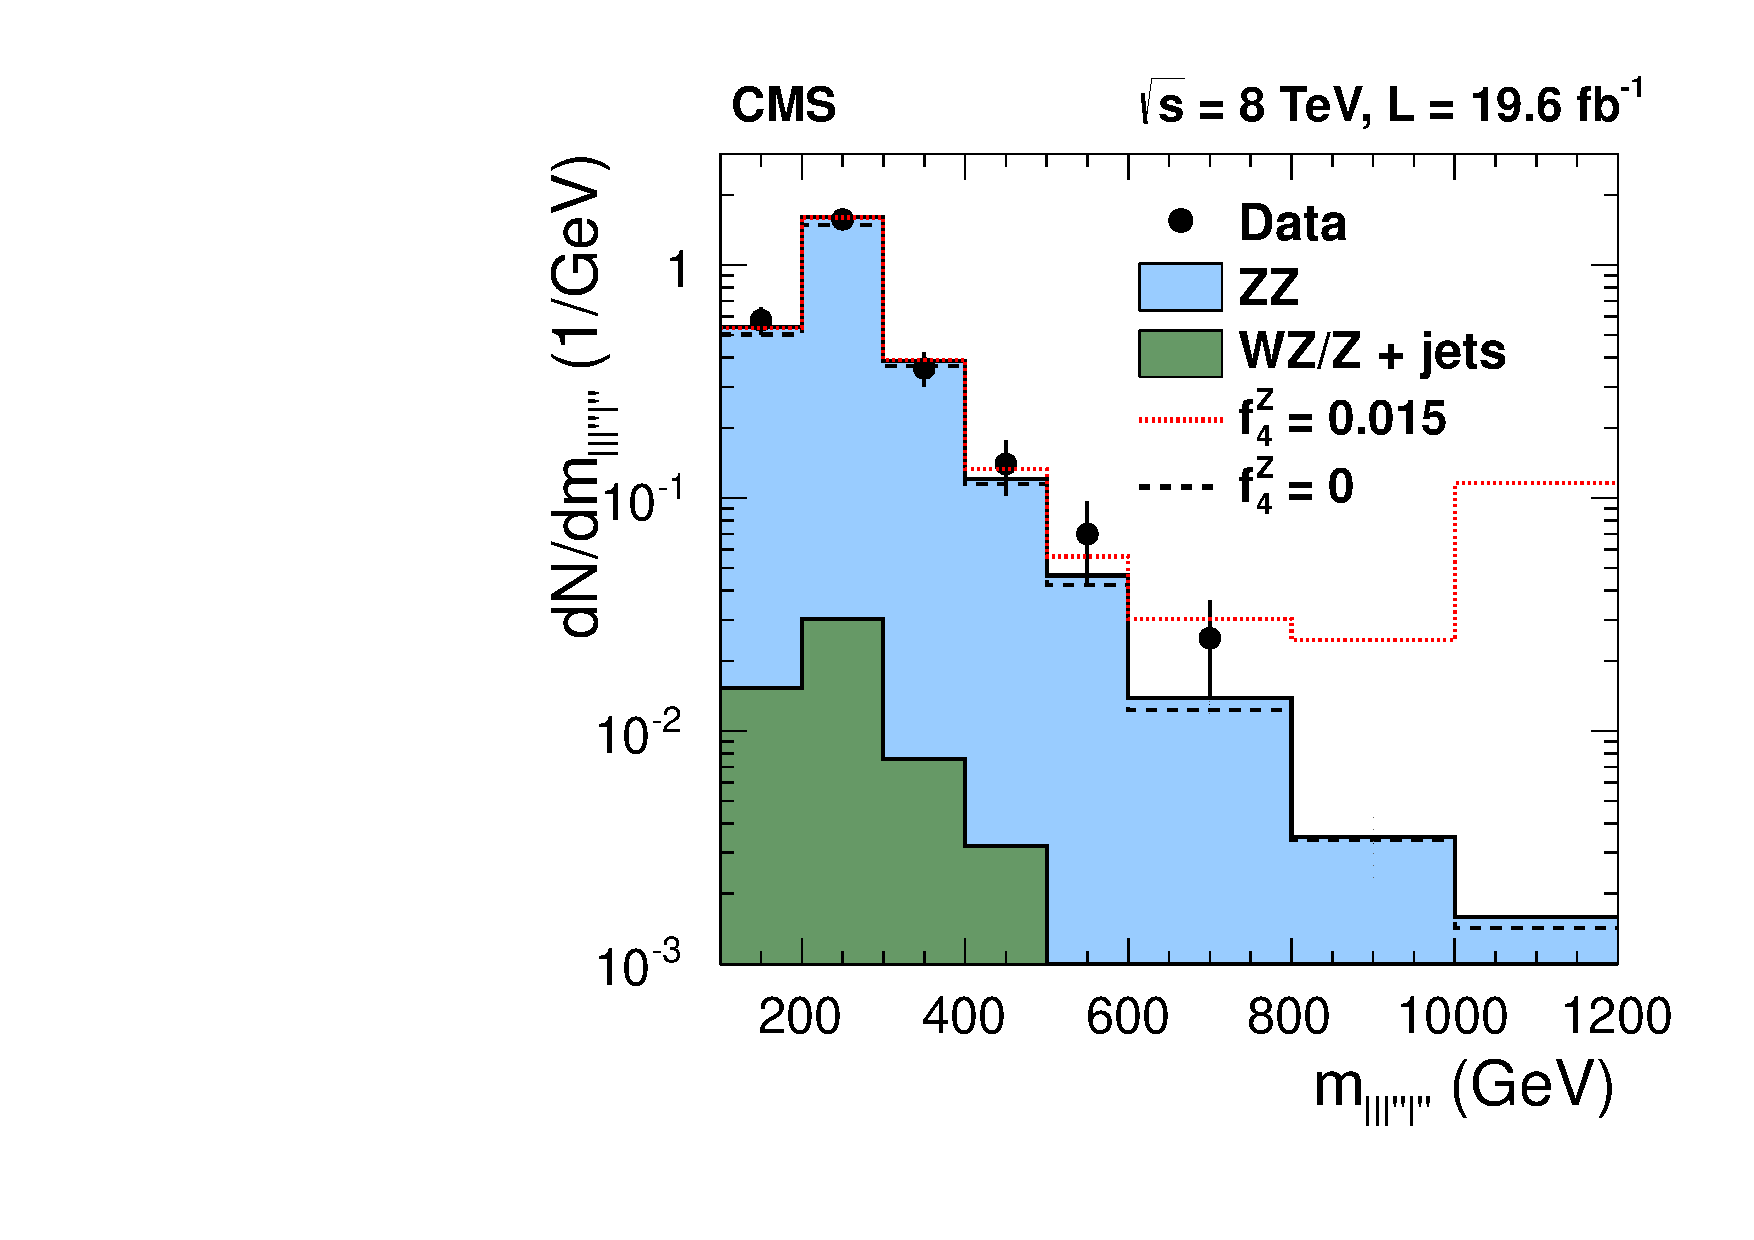
\includegraphics[width=0.9\textwidth]{figures/sss-inclboson-diboson-zzprod-zzinvmass.pdf}
  \caption{ Distribution of the four-lepton reconstructed mass for the combined $4e$, $4\mu$, and $2e2\mu$ channels from CMS~\cite{Khachatryan:2014dia}. Points represent the data, the shaded histogram labeled $\ZZ$ represents the predictions for $\ZZ$ signal, the histograms labeled $\WZ$/$\Z$+jets shows background estimated form data. The dashed and dotted histograms indicate the SM expectation (f4Z = 0) and in the presence of an ATGC (f4Z = 0.015) with all the other anomalous couplings set to zero. The last bin includes all entries with masses above 1000 GeV.
}
\label{fig:sss-inclboson-diboson-zzprod-zzinvmass}
\end{center}
\end{figure}

Both experiment publish 95\% CL limits on ATGC without form factors in the $\ll\ll$ 
and $\ll\vv$ channels. The results are in agreement with the SM and 
summarized in Figure~\ref{fig:sss-inclboson-diboson-zzprod-aTGC_naTGCf} 
taken from Ref. \cite{aTGCplots}. The precision of the LHC results is driven by the steep increase of 
sensitivity with higher centre-of-mass energy
and are about 2 orders of magnitude better compared to the 
combined LEP result~\cite{LEP-comb-2002}.  
% FIGURE COMPARISON OF ZZ NTGC
% https://twiki.cern.ch/twiki/bin/view/CMSPublic/PhysicsResultsSMPaTGC
% M Herndon
% FETCHED 34RD JULY 2015
\begin{figure}[htbp]
  \begin{center}
  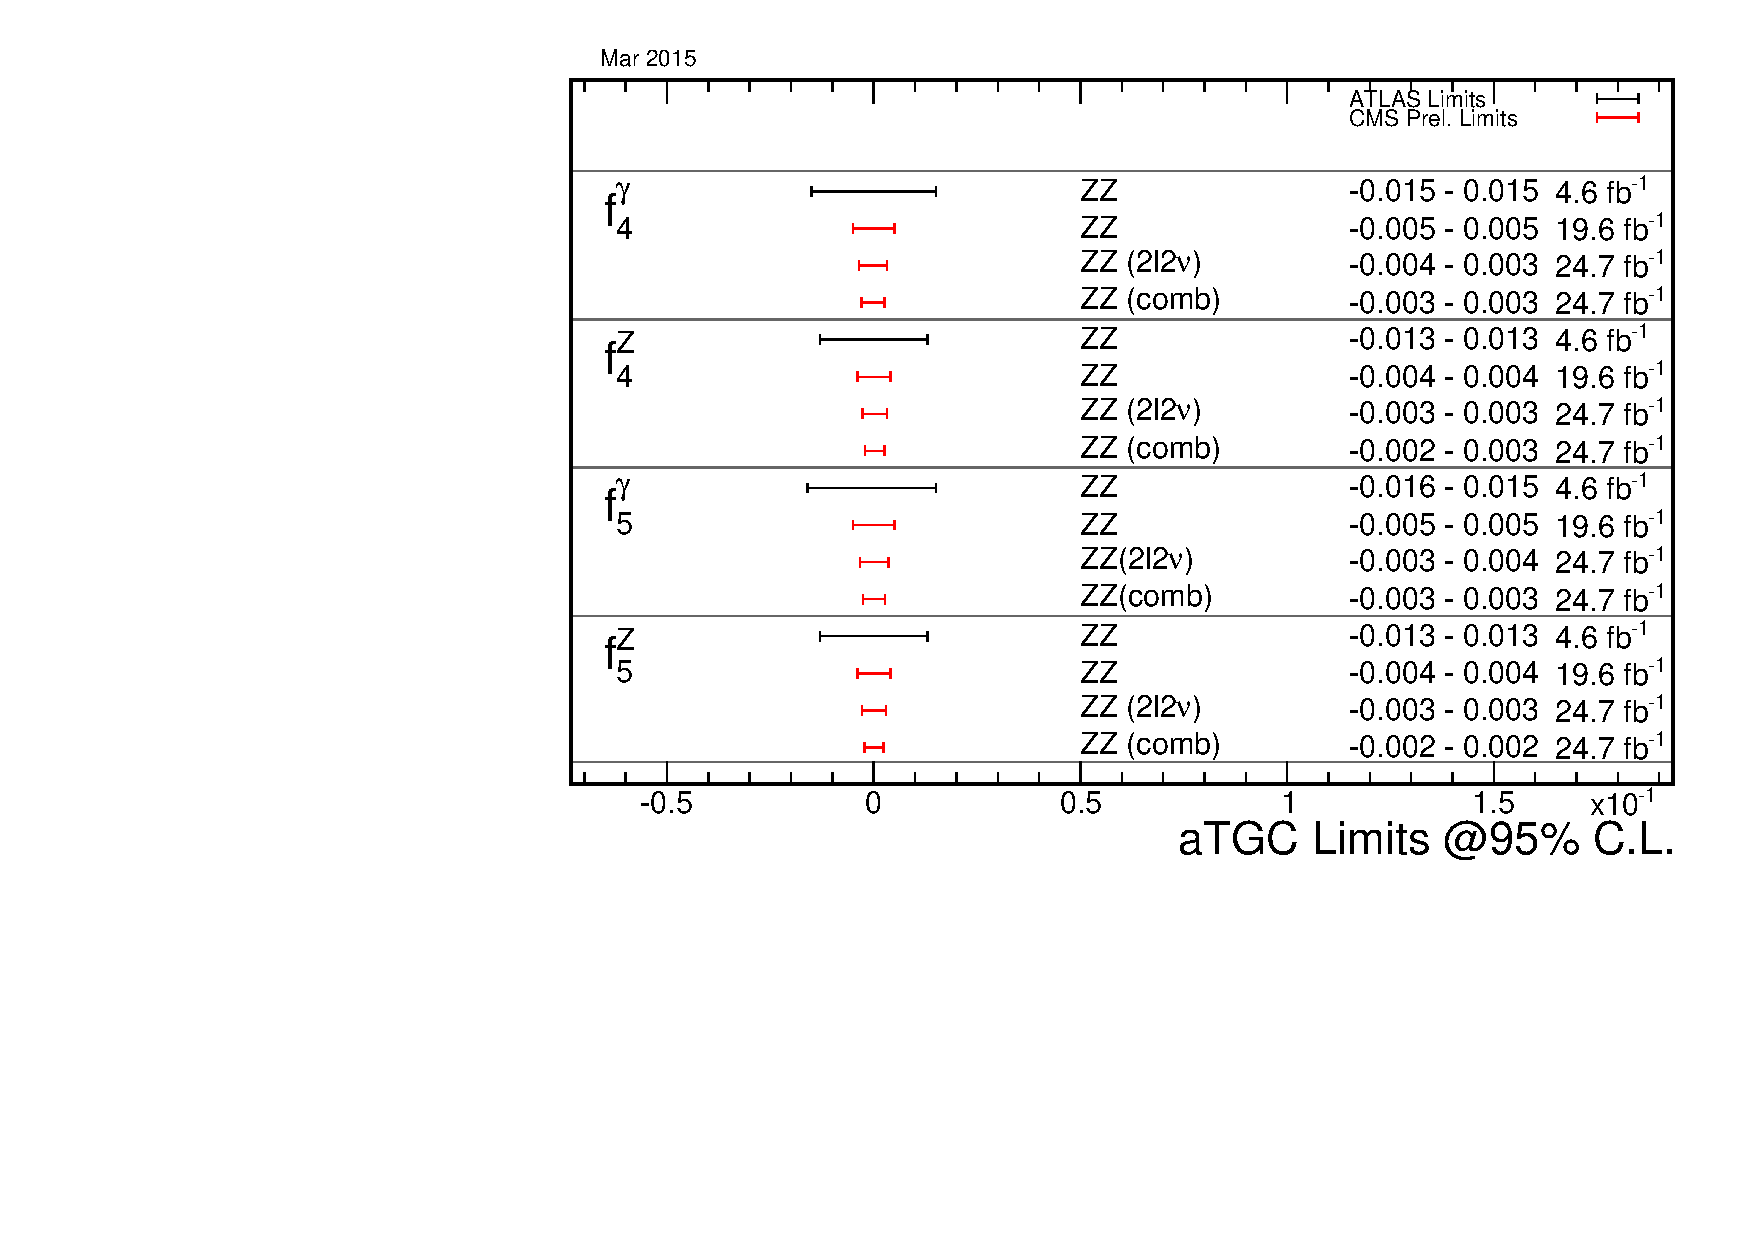
\includegraphics[width=0.9\textwidth]{figures/sss-inclboson-diboson-zzprod-aTGC_naTGCf.pdf}
  \caption{ Comparison of the limits on \ffourv{} and \ffivev{} from ATLAS and CMS in the $\ll\ll$ and $\ll\vv$
  channel at 7 and $8\TeV$.}
\label{fig:sss-inclboson-diboson-zzprod-aTGC_naTGCf}
\end{center}
\end{figure}









%ATLAS ZZ 7 TeV~\cite{Aad:2012awa}
%CMS ZZ4l 8 TeV~\cite{Khachatryan:2014dia}
%CMS ZZ4l 7 TeV~\cite{Chatrchyan:2012sga}
%CMS ZZ2l2nu 7+8 TeV~\cite{Khachatryan:2015pba}




\subsection{Inclusive tri-boson production}

ATLAS $W\gamma\gamma$~\cite{Aad:2015uqa}

CMS WVgamma 8 TeV~\cite{Chatrchyan:2014bza}

\section{Exclusive boson production}
\subsection{Exclusive single boson production, vector-boson fusion}

ATLAS VBF Z 7 TeV~\cite{Aad:2014dta}

CMS VBF Z 7 TeV~\cite{Chatrchyan:2013jya}

CMS VBF Z 8 TeV~\cite{Khachatryan:2014dea}

\subsection{Exclusive di-boson production, vector-boson scattering}

ATLAS SSWW 8 TeV~\cite{Aad:2014zda}

CMS WWexcl 7 TeV~\cite{Chatrchyan:2013foa}

CMS SSWW 8 TeV~\cite{Khachatryan:2014sta}

\section{Electroweak (precision) tests of the standard model}
\subsection{Test of tri-boson vertex}

ATLAS Wgamma Zgamma 7 TeV~\cite{Aad:2013izg}

ATLAS WW 7 TeV~\cite{ATLAS:2012mec}

ATLAS $WW+WZ$ cross section 7 TeV~\cite{Aad:2014mda}

ATLAS WZ 7 TeV~\cite{Aad:2012twa}

ATLAS ZZ4l,ZZ2l2v 7 TeV~\cite{Aad:2012awa}

CMS ZZ4l 8 TeV~\cite{Khachatryan:2014dia}

CMS ZZ4l 7 TeV~\cite{Chatrchyan:2012sga}

CMS WW2l2n 7 TeV~\cite{Chatrchyan:2013yaa}

CMS WWlnjj 7 TeV~\cite{Chatrchyan:2012bd}

CMS WW2l2n 8 TeV (CMS-PAS-SMP-14-016, to be published)

CMS Wgamma/Zgamma 7 TeV~\cite{Chatrchyan:2013fya}

CMS Znngamma 7 TeV~\cite{Chatrchyan:2013nda}

CMS Zgamma 8 TeV~\cite{Khachatryan:2015kea}

CMS ZZ2l2nu 7+8 TeV~\cite{Khachatryan:2015pba}

\subsection{Test of tetra-boson vertex}

ATLAS $W\gamma\gamma$ 8 TeV~\cite{Aad:2015uqa}

ATLAS SSWW 8 TeV~\cite{Aad:2014zda}

CMS WVgamma 8 TeV~\cite{Chatrchyan:2014bza}

CMS WWexcl 7 TeV~\cite{Chatrchyan:2013foa}

CMS SSWW 8 TeV~\cite{Khachatryan:2014sta}

\subsection{Z AFB and sin thetaW}

ATLAS weak mixing angle~\cite{Aad:2015uau}

CMS weak mixing angle~\cite{Chatrchyan:2011ya}

CMS Drell--Yan AFB 7 TeV~\cite{Chatrchyan:2012dc}

CMS Drell--Yan AFB 8 TeV (CMS-PAS-SMP-14-004, to be published)

\subsection{W mass}

\section{Summary}


ATLAS~\cite{Aad:2008zzm}
CDF~\cite{Abulencia:2005ix}
CMS~\cite{CMSdetector}
D0~\cite{Abazov:2005pn}
LHCb~\cite{Alves:2008zz}

CDF Z asymmetry muon~\cite{Aaltonen:2014loa}
CDF Z asymmetry electron~\cite{Aaltonen:2013wcp}
CDF W mass PRD~\cite{Aaltonen:2013vwa}
CDF W mass PRL~\cite{Aaltonen:2012bp}

D0 W asymmetry electron~\cite{Abazov:2013dsa}
D0 W asymmetry muon~\cite{Abazov:2013rja}
D0 W mass PRD~\cite{D0:2013jba}
D0 W mass PRL~\cite{Abazov:2012bv}

CDF+D0 W mass combination~\cite{Aaltonen:2013iut}

Snowmass electroweak~\cite{Baak:2013fwa}

Wmass PDF~\cite{Bozzi:2011ww}

\ack
Acknowledgments go here. 

\bibliographystyle{iopart-num}
\bibliography{ewkrun1_master}

\end{document}

